\documentclass[12pt]{article}

\usepackage{amsfonts}
\usepackage{amssymb}
\usepackage{epsfig}
\usepackage{enumerate}
\usepackage[letterpaper,text={6.5in,9in}]{geometry}
\newcommand{\bs}{\bigskip \noindent}
\newcommand{\noi}{\noindent}
\newcommand{\vs}[1]{\vspace{#1}\noindent}
\newcommand{\im}{\item}
\newcommand{\hs}{\hspace}
\newcommand{\pb}{\pagebreak\noindent}
\newcommand{\be}{\begin{enumerate}}
\newcommand{\ee}{\end{enumerate}}
\newcommand{\bi}{\begin{itemize}}
\newcommand{\ei}{\end{itemize}}
\newcommand{\R}{{\mathbb R}}
\newcommand{\Z}{{\mathbb Z}}
\newcommand{\Q}{{\mathbb Q}}
\newcommand{\Lra}{\Leftrightarrow}
\pagestyle{empty}

\begin{document}

Graph the quadratic function with the characteristics below.  Be sure to label the appropriate points on the graph.
	\begin{itemize}
	\item	Vertex: $(-4,1)$  $y=-.25(x+2)(x+6)$
	\item $y$-intercept: $y=-3$ 
	\item $x$-intercepts: $x=-2,-6$
	\item Axis of symmetry: $x=-4$
	\end{itemize}
	\begin{center}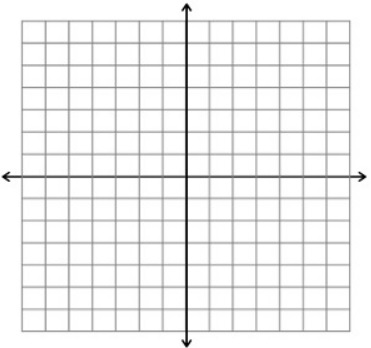
\includegraphics{fig-graphpaper.png}\end{center}\begin{center}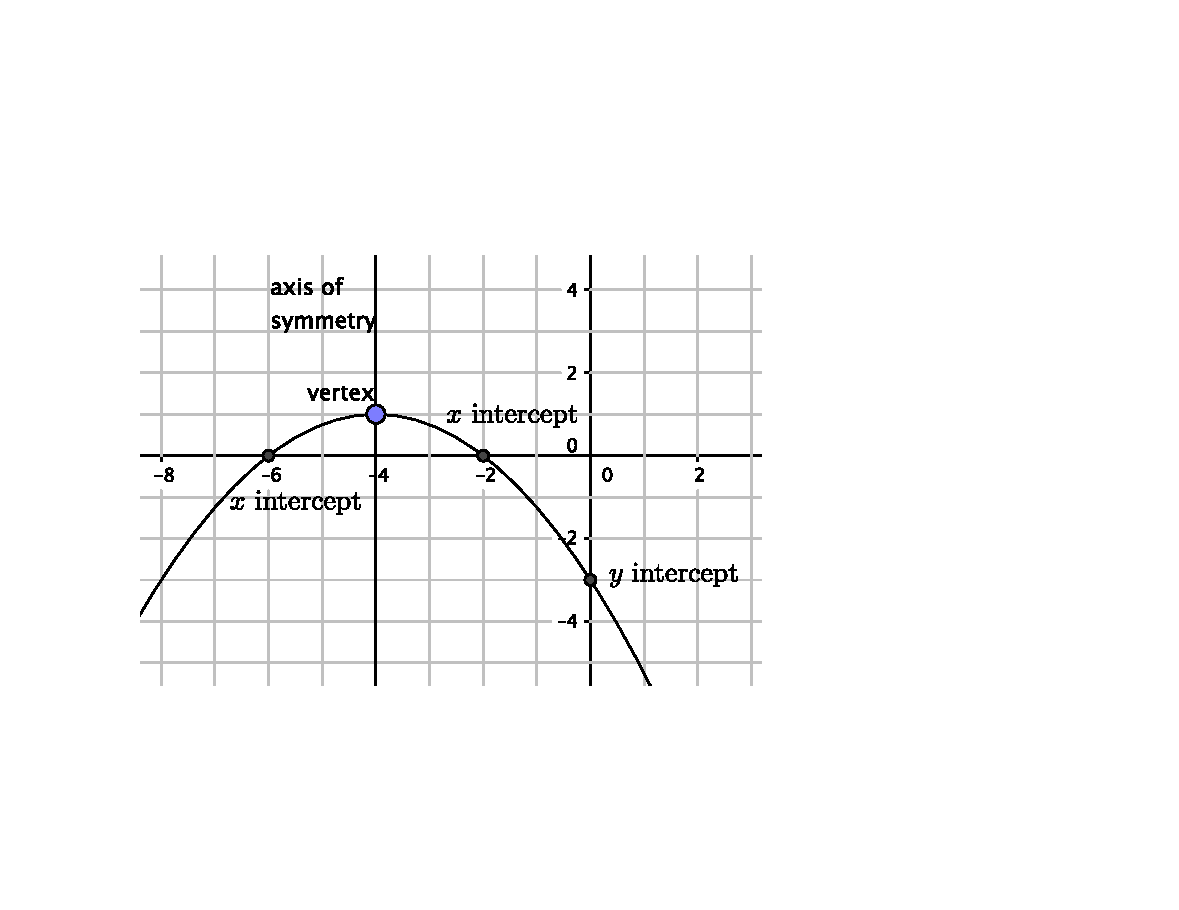
\includegraphics{fig100-18_5-a-answer}\end{center}
\end{document}
